\section{Complexity Considerations}
\label{sec:complexity}
% ================================================================================


 
As can be seen from the specification of the test cases $U_F(k)$ 
(see Section~\ref{sec:finitecompletefails}), the number of
executions ending in a $\epass$-event corresponds to the number $\ell$ of traces $s$
of $P$ with length equal to\footnote{In this estimation, we disregard
the case where the test
terminates earlier due to entering branch (\ref{eq:ufb}).} $k$,
multiplied by the number $h$ of minimal hitting sets in
$\minhits(P/s)$. For the tests $U_T(k)$ verifying trace refinement (see Section~\ref{sec:finitecomplete}), the number of executions equals $\ell$, since
there is no equivalent in $U_T(k)$ 
to checking different hitting sets in the last step of a 
test execution.



% -------------------------------------------------------------------------
\subsection{Estimation of $\ell$}
The first factor $\ell$
has worst-case upper bound $\ell\le \card{\Sigma}^k$. As an example, where this upper bound 
is really met, consider the reference process
\[
RUN(\Sigma) = e:\Sigma \then RUN(\Sigma).
\]
The normalised transition graph of this process has a single state, and its initials
are $[RUN(\Sigma)]^0 = \Sigma$. Therefore, the associated test process $U_F(k)$ can 
never enter branches (\ref{eq:ufa}) and (\ref{eq:ufb}), but there are exactly 
$\card{\Sigma}^k$ different traces of length $k$ exercising branch (\ref{eq:ufc})
for each of their events.

% -------------------------------------------------------------------------
\subsection{Estimation of $h$}
Given a set $\minaccs(P/s) = \{ A_1,\dots, A_\alpha \}$ of   minimal
acceptances, the cardinality   $h = \minhits(P/s)$ has the upper bound
\[
h \le \binom{n}{\lfloor\frac{n}{2}\rfloor}, \quad \text{where $n = \card{\Sigma}$.}
\]
This follows from Theorem~\ref{th:sperner} and the fact that $\minhits(P/s)$ is a 
Sperner Family, as introduced in Section~\ref{sec:hit}. The next theorem shows that this
upper bound can really be reached by collections of minimal hitting sets.

\begin{theorem}
\label{th:upperboundh}
Let $n\ge 2$ be any positive integer and $\Sigma$  any finite set of cardinality $n$.
Let $C\subseteq 2^\Sigma$ be any collection of  subsets of $\Sigma$. Then  
\[
\text{max}\{\card{\text{minHit}(C)}~|~C\subseteq 2^\Sigma\}=\binom{n}{\lfloor\frac{n}{2}\rfloor}
\]
\end{theorem}
\begin{proof}
For any subset  $B$  of $\Sigma$, define  $A_{B}:=\Sigma\setminus B$.
Define 
$$
C=\{A_{B}~|~ B\subseteq \Sigma, \card{B} < \lfloor\frac{n}{2}\rfloor\}.
$$
Let $H$ be any minimal Hitting set of $C$. Then $H$ contains at least $\lfloor\frac{n}{2}\rfloor$ elements, because 
otherwise there existed an $A_{H}\in C$ with $A_H\cap H=\varnothing$. 
Since $\card{A_{B}}=n-\card{B}>n-\lfloor\frac{n}{2}\rfloor$, for any $B\subseteq \Sigma$ with $\card{B}< \lfloor\frac{n}{2}\rfloor$, we conclude that
 any  subset of $\Sigma$  with at least $\lfloor\frac{n}{2}\rfloor$ elements 
 has a non-empty intersection with all  $A_B\in C$.  
 The number of subsets in $\Sigma$ with exactly $\lfloor \frac{n}{2}\rfloor$ elements
 is $\binom{n}{\lfloor\frac{n}{2}\rfloor}$.
Thus $\card{\text{minHit}(C)} \ge \binom{n}{\lfloor\frac{n}{2}\rfloor}$, and 
Theorem~\ref{th:sperner} yields $\card{\text{minHit}(C)} = \binom{n}{\lfloor\frac{n}{2}\rfloor}$.
\xbox
\end{proof}


To get an approximation of the maximal size of $\minhits(P/s)$ for large $n$, recall
Stirling's approximation~\cite[p.~112]{Graham:1994:CMF:562056}
\[
m! \approx \sqrt{2\pi m} \cdot \big( \frac{m}{e} \big)^m, \quad\text{where $e$ denotes the Euler Number.}
\]
Applying this approximation to the   case where $n = \card{\Sigma}$ is even and $m = (n/2)$  
results in
\[
h \le \binom{2m}{m} \approx \frac{4^m}{\sqrt{\pi m}} = 
\frac{2^\card{\Sigma}}{\sqrt{2\pi \card{\Sigma}}}.
\]
%
We note that, due to this approximation result, 
$h$ is   smaller than $2^{\card{\Sigma}}-1$, the cardinality of the 
non-empty subsets of $\Sigma$.

% -------------------------------------------------------------------------
\subsection{Upper Bounds of Test Executions for Checking Failures Refinement}
According to  Theorem~\ref{th:failurestest}, we need to execute the tests $U_F(k)$ for
$k = 0,\dots,(pq-1)$; this results in a worst-case bound defined below, where
we use the formula for the sum of the geometric progression.
%
\[
h\cdot \big( \frac{1-\card{\Sigma}^{pq}}{1-\card{\Sigma}} \big),\
 \text{or, asymptotically,}\  O(\frac{2^\card{\Sigma}}{\sqrt{2\pi \card{\Sigma}}}\cdot\card{\Sigma}^{(pq-1)}).
 \]
%
From Theorem~\ref{th:upperboundh} we know that the worst-case bound for $h$
above cannot be further improved, since the full collection of minimal
hitting sets needs to be checked to verify $conf$. The
authors of~\cite{Hennessy:1988:ATP:50497} and
\cite{DBLP:conf/icfem/CavalcantiG07} suggest to test {\it every} non-empty
subset of $\Sigma$ whose events cannot be completely refused in a given
process state of the reference model; this leads to a worst-case estimate of
$2^{\card{\Sigma}}-1$ for the number of different sets to be offered to the SUT in
the last step of the test execution, so our approach reduces the number of
test executions in comparison
to~\cite{Hennessy:1988:ATP:50497,DBLP:conf/icfem/CavalcantiG07} by a factor of
$1/{\sqrt{2\pi \card{\Sigma}}}$.

In Fig.~\ref{fig:minhita}, the reduction is visualised by a function plot of
$2^{\card{\Sigma}}$ versus $\frac{2^\card{\Sigma}}{\sqrt{2\pi \card{\Sigma}}}$.



% .....................................................................................
 \begin{figure}
 %%\hspace*{-40mm}
 \begin{center}
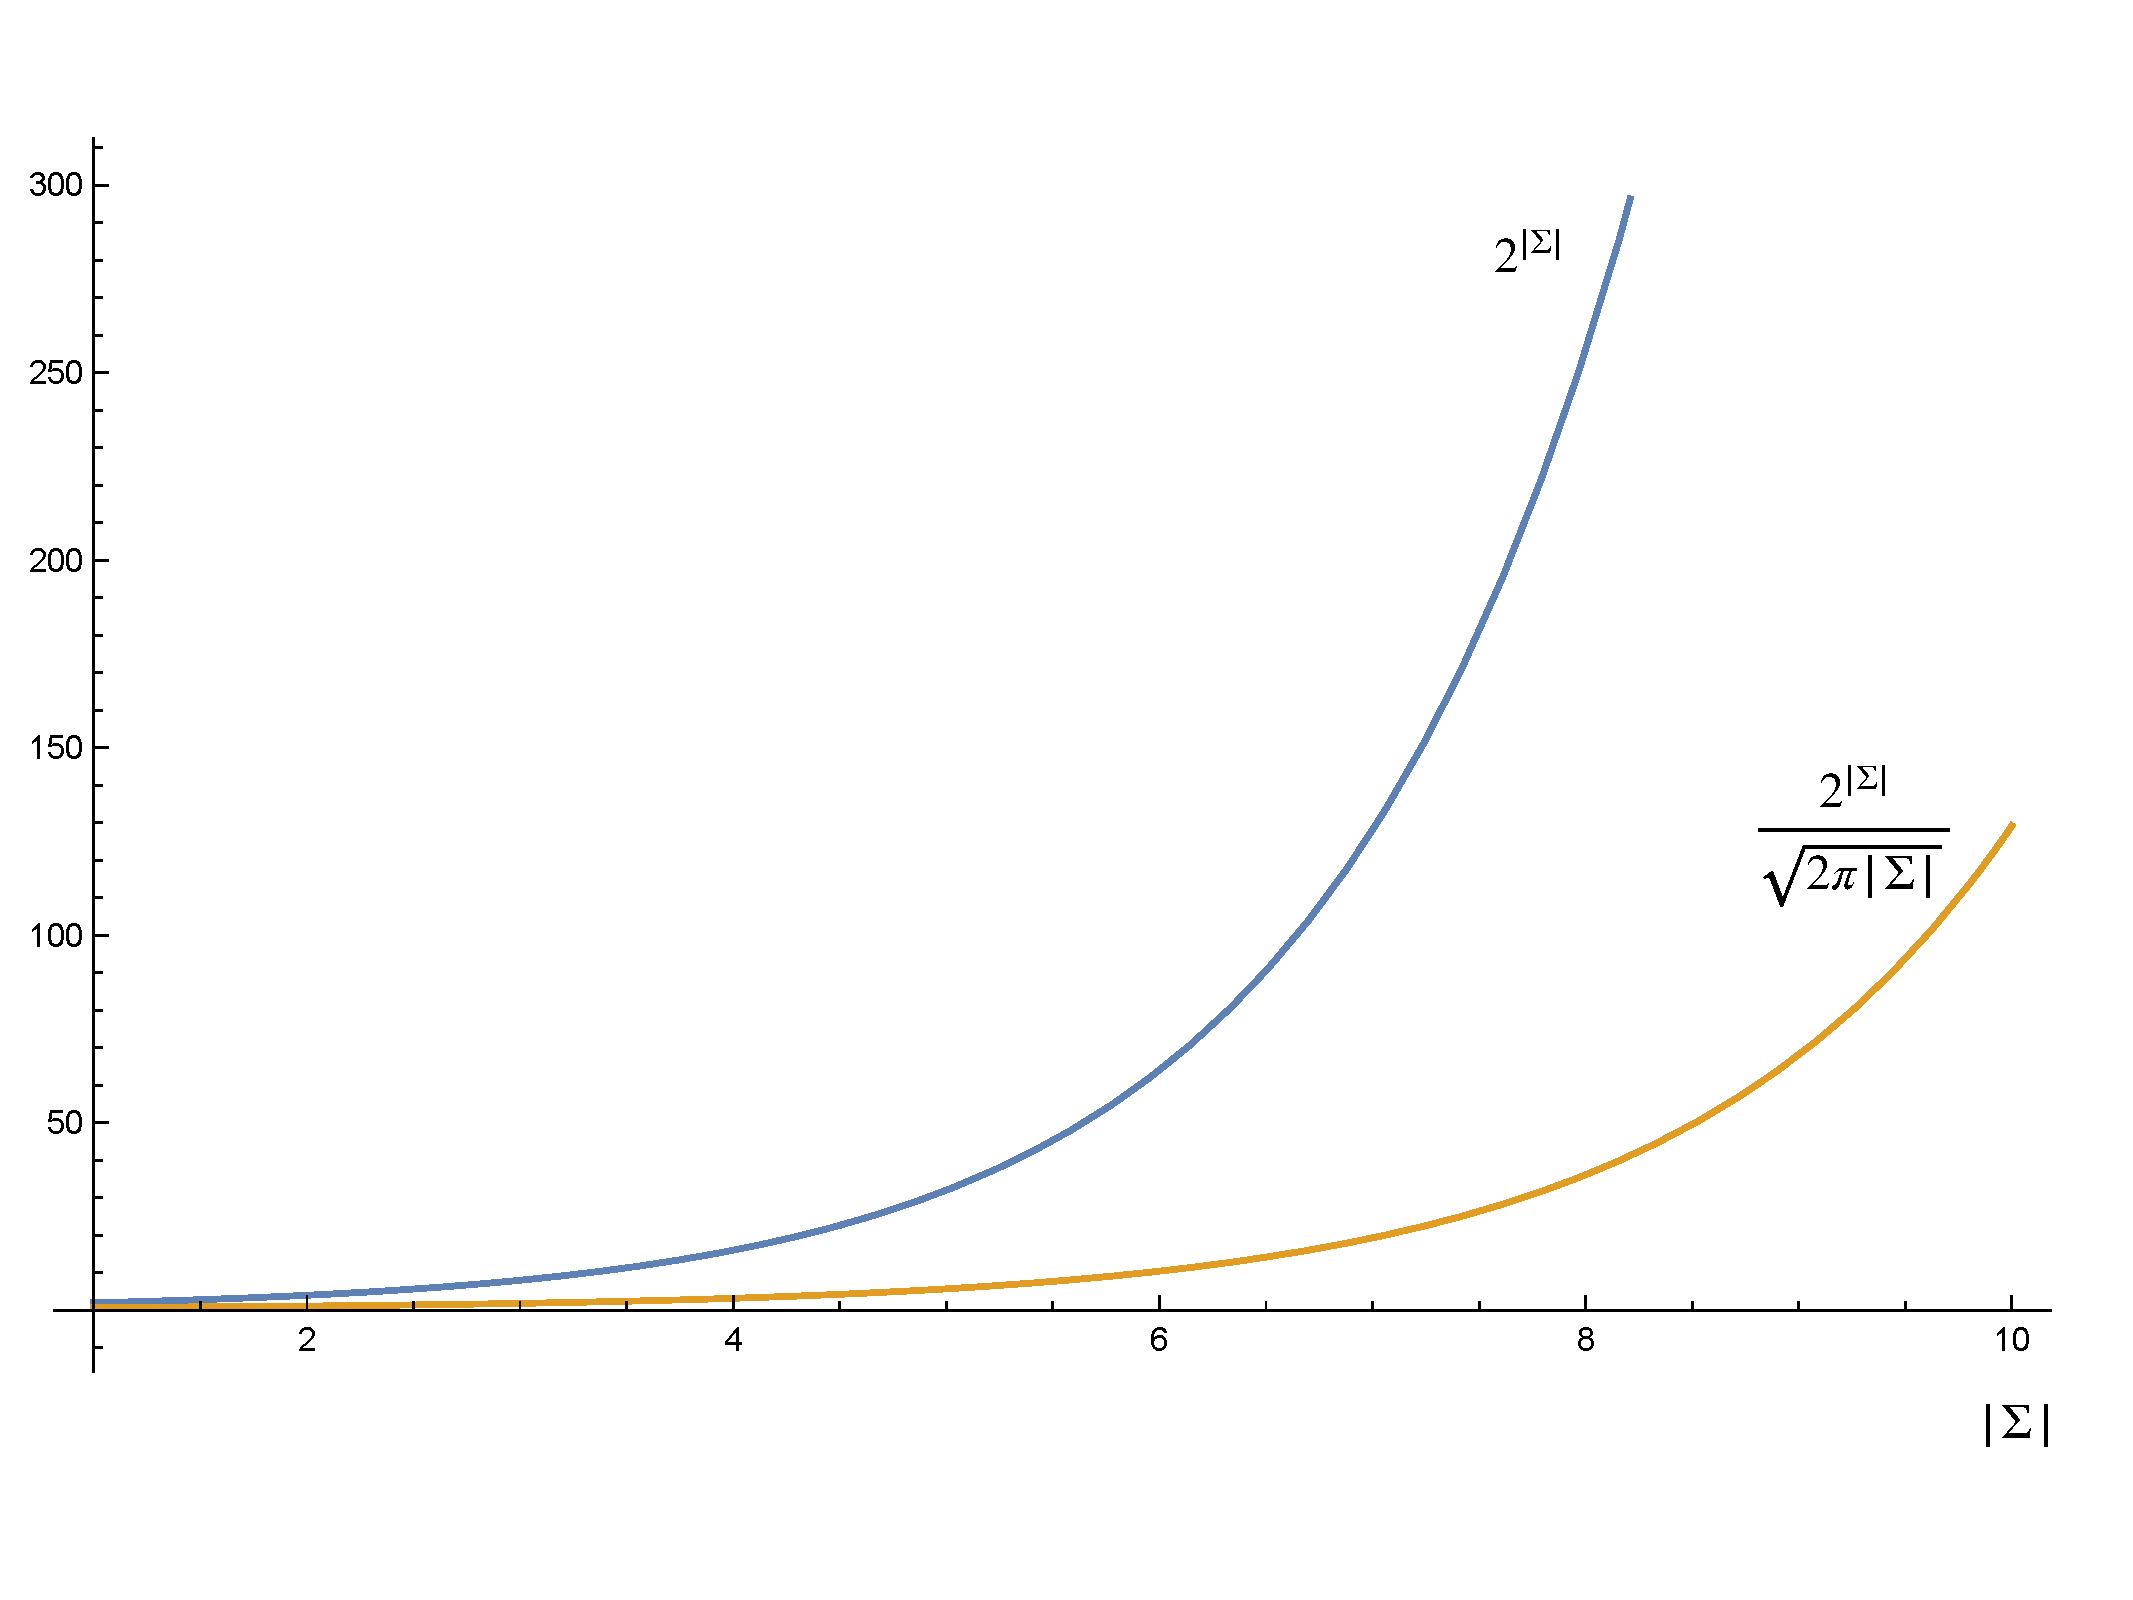
\includegraphics[width=.8\textwidth]{minhit-fig.pdf}
\end{center}
\vspace*{-10mm}
\caption{Function plot $2^{\card{\Sigma}}$ versus $\frac{2^\card{\Sigma}}{\sqrt{2\pi \card{\Sigma}}}$.}
 \label{fig:minhita}
 \end{figure}
% .......................................................................................

% -------------------------------------------------------------------------
\subsection{Upper Bounds of Test Executions for Checking Trace Refinement}

According to Theorem~\ref{th:tracetest}, a complete test suite checking trace
refinement just contains the adaptive test case $U_T(pq-1)$. As derived for $U_F(k)$
above, the number of executions performed by $(Q\parallel[\Sigma] U_R(pq-1))$ 
is bounded by $\card{\Sigma}^{pq-1}$.


% -------------------------------------------------------------------------
\subsection{Upper Bound $pq$ for the Maximal Length of Test Traces}

According to Theorem~\ref{th:failurestest}, the tests $U_F(k)$ need to be executed for 
$k = 0,\dots,pq-1$ to guarantee completeness. This means that the SUT is verified 
with test traces up to, and including, length $pq$:
recall from the test specification, branch (\ref{eq:ufa}), that $U_F(k)$ will accept
all traces $s.e$ with $s\in\trc(P), \#s = k, e\not\in\trc(P/s)$, so erroneous trace
up to length $k+1$ are detected.
It is interesting to  investigate
whether this maximal length is really necessary, or whether one could elaborate
alternative complete test strategies where the SUT is tested with shorter traces only. 
Indeed, an example  presented in~\cite[Exercise~5]{PeleskaHuangLectureNotesMBT} 
shows that when testing for equivalence of deterministic FSMs, it is sufficient to
test the SUT with traces of significantly shorter length.

The following example, however, shows that the maximal length $pq$ is really required 
when testing for refinement.
\begin{example}\label{ex:pq}
Consider the CSP reference process $P$ and an erroneous implementation $Q$ specified
as follows.
\begin{eqnarray*}
P & = & a \then P_1 \intchoice b \then P_1 \intchoice c \then P_1
\\
P_1 & = & a \then P \extchoice b\then P
\\ & &  \\
Q & = & a\then Q_1 \extchoice b\then Q_1
\\
Q_1 & = & a\then Q_2 \extchoice b\then Q_2
\\
Q_2 & = & a\then Q \intchoice b\then Q
\end{eqnarray*}
Obviously, $P$'s normalised transition graph has 2 nodes, 
while $Q$'s graph has 3.
It is easy to see (and can be checked with FDR4) that $P\lessdet_T Q$, but 
$\neg(P\lessdet_F Q)$. Furthermore, it can also be shown using the FDR4 tool that
the ``test passed condition'' 
\[
(\epass\then\Stop) \lessdet_F (Q\parallel[\Sigma] U_F(k))\hide \Sigma
\]
holds for $U_F(0),\dots,U_F(4)$, but fails for $U_F(5)$. This means that the
non-conformance of $Q$ cannot be detected by any test trace of length 
less or equal to 5, but is revealed (as expected from Theorem~\ref{th:failurestest})
by a trace of length 6, because the last event offered by the test $U_F(5)$ is 
refused by $Q$.
\xbox
\end{example}
%
Generalising Example~\ref{ex:pq}, it can be shown that for any pair 
$2\le p,q \in\mathbb{N}$,  
there exist reference processes with $p$ states
and implementation processes with $q$ states, such that 
a violation of the trace refinement property
can only be detected with a trace of length $pq$. This is proven in the following 
theorem.

\begin{theorem}\label{th:maxtracelen}
Let $2\le p,q \in\mathbb{N}$. Then there exists a reference process $P$ and an
implementation process $Q$ with the following properties.
\begin{enumerate}
\item $G(P)$ has $p$ states.
\item $G(Q)$ has $q$ states.
\item $P\not\lessdet_T Q$.
\item $\forall s\in\trc(Q): \#s < pq\implies s\in\trc(P)$.
\end{enumerate}
As a consequence, the upper bound $pq$ for the length of traces to be tested when checking for failures refinement cannot be reduced without losing the test suite's completeness property.
\end{theorem}
\begin{proof}
Given $2\le p,q \in\mathbb{N}$, define reference process $P$ and implementation process $Q$
over alphabet $\Sigma =\{ a,b\}$ as follows.
\begin{eqnarray*}
P & = &  P(0) 
\\
P(k) & = & \big( a \then P(k) \big) \extchoice (k < p-1) \& \big( b \then P(k+1)\big)
\\ 
Q & = & Q(0)
\\
Q(k) & = & (k < q-1) \& \big( a \then Q(k+1)    \big) \extchoice 
( k = q-1)\& \big( a\then Q(0) \extchoice b\then Q(0)  \big)
\end{eqnarray*}
Using regular expression notation, the traces of $P$ can be specified as
\[
\trc(P) = \prefs\big(  (a^*b)^{p-1}a^* \big),
\]
where $\prefs(M)$ denotes the set of all prefixes of traces in $M\subset\Sigma^*$, 
including the traces of $M$ themselves.
The traces of $Q$ can be specified by
\[
\trc(Q) = \prefs\big( (a^{q-1}(a|b))^*  \big).
\]
It is easy to see that $\trc(Q)\not\subseteq\trc(P)$; 
for example, the trace $(a^{q-1}b)^p$ is in
$\trc(Q)\setminus\trc(P)$.

Let $s \in\trc(Q)$ be any trace of length $\#s = pq-1$. Then $s$ can be represented 
by $s = (a^{q-1}(a|b))^{p-1}a^{q-1} \in \prefs\big( (a^{q-1}(a|b))^*  \big)$. 
Then $s$ is also an element of $\trc(P)$, because $(a^{q-1}(a|b))^{p-1}a^{q-1}$ 
is also contained in $\prefs\big(  (a^*b)^{p-1}a^* \big)$: this is easy to see, since
$\prefs\big(  (a^*b)^{p-1}a^* \big)$ contains all finite sequences of $a$-events, 
where at most $p-1$ events $b$ have been inserted.
\xbox
\end{proof}

Since Theorem~\ref{th:maxtracelen} just states that a violation of trace refinement
may remain undetected if only traces shorter than $pq$ are checked during tests, 
it can also be applied to our trace refinement tests. Therefore, 
test suites $\{ U_T(z) \}$ with $z<pq-1$ are no longer complete.


It is discussed in Section~\ref{sec:conc} how the number of test traces to be executed 
by complete test suites for failures or tarce 
refinement   can still be reduced {\it without} reducing 
the maximal length.

% =================================================================================